\section{The Benchmark: Computation of Shapley Effects} \label{comp_shap}

This section introduces Shapley effects for sensitivity analysis. Shapley effects will serve as a benchmark for evaluating the performance of the sensitivity measures derived by the Morris method.

\subsection{Shapley Values in Economics}

The Shapley value is a concept from cooperative game theory, introduced by \citet{S53}. It is a value that informs about how to fairly distribute the profit of a product that was created by a team effort. Fairly here means that any player receives as much of the gain as he or she contributed to the team effort. As individual contributions are not directly observed, \citet{S53} proposes the following value. The Shapley value ensures that every individual receives at least as much as if he or she had if acted independently \citep{IP19}.

Consider a game with $k$ players, where $K$ denotes the set of all players, the grand coalition. A coalition is a subset $J \subset K$. Let $- J$ denote the complement set of $J$, i.e. $- J = K \setminus{J}$. The corresponding game is defined by a coalition value function that maps each coalition $J$ to the value attained by this coalition, i.e. $val: 2^K \to \mathbb{R}_{\geq 0}$, where $2^K$ denotes the power set of $K$, i.e. the set of all subsets of $K$. It is generally assumed that $val(\emptyset) = 0$. The following definition is strongly inspired by the one found in \citet{PRB20}:

\begin{definition}

Given a coalition worth function $\text{val}$, the marginal contribution of player $i$ joining coalition $J$ is $\text{mar}(J, i)=\text{val}(J \cup \{i\}) - \text{val}(J)$. The Shapley value is then defined as
\begin{equation*}
\begin{split}
\phi_{i} (\text{val})& = \sum_{J \mid i \notin J} \frac{\vert J \vert ! (k - \vert J \vert - 1) ! }{ k !} (\text{val}(J \cup \{i\}) - \text{val}(J)) \\
& = \frac{1}{k} \sum_{J \mid i \notin J} \binom{k-1}{\vert J \vert}^{-1} \text{mar}(J, i).
\end{split}
\end{equation*}

\end{definition}

In other words, we consider every coalition of players and evaluates by how much the inclusion of player $i$ increases the overall profit of the coalition. This is achieved by subtracting the value generated by the members of coalition $J$ from the value created by the larger coalition that includes coalition $J$ and player $i$. In the context of a game, the marginal value for each coalition is divided among all members of this coalition, e.g. if the coalition has one member only, the entire marginal value is gained by this player. We can also interpret the Shapley value as the expected payoff from joining a coalition or from leaving the complementary coalition \citep{PRB20}.

\citet{S53} shows that $\phi_i$ is the only value satisfying all the following four axioms at the same time. Note that Shapley values normalised by total profit are considered.

\begin{itemize}
    \item Pareto efficiency: $\sum_{i=1}^{k}\phi_i=1$.
	\item Symmetry: If $val(J \cup {i})=val(J \cup {j})\ \forall\ J \subseteq K \setminus{\{i, j\}}$, then $\phi_i = \phi_j$.
	\item Linearity: $\phi_i(val_1 + val_2)=\phi_i(val_1)+\phi_i(val_2)$.
	\item Null-player: If $\forall J,\ mar(J, i) = 0$ holds then $\phi_i(val) = 0$.
\end{itemize}

Pareto efficiency ensures that nothing of the profit gained by the team is wasted. Normalised by the total profit, the Shapley value gives the share attained by each individual in the game. Symmetry implies that all players who contributed the same to the common product, receive the same payoff, reflecting the meritocratic principle. The null-player axiom ensures that players who do not contribute to the team effort at all do not receive any share of the profits. Especially axioms 1 and 4 are desirable in the context of the Shapley value as a variance-based sensitivity measure, as further discussed in the following subsection.

\subsection{Variance-based Sensitivity Analysis} \label{var_based_sa}

There are several purposes for which we can apply sensitivity methods in general. Note, that in sensitivity analysis we refer to input variables by the term factors \citep{R21}. In their textbook, \citet{STC04} summarise the following four possible objectives of sensitivity analysis.

Factors Prioritisation (FP): In the FP setting, we determine on which inputs applied, uncertainty reduction results into the largest reduction in output uncertainty. Sensitivity analysis determines the importance of an input variable. Applied to all inputs, we can derive a ranking of all inputs in order of importance. FP can guide research by prioritising inputs. Inputs are identified for which better experimental measurement can reduce output uncertainty the most, supposing that additional information costs the same for alle inputs.

Factors Fixing (FF): The FF setting allows us to determine the least influential inputs. These can then be fixed at a specific value while losing only a minimum of information in the model output. FF can also be seen as input screening. We would want to fix the least influential inputs to reduce dimensionality of the model and thus the complexity and computational burden.

Variance Cutting (VC): VC informs about which inputs to fix to arrive at a certain desired value of the output variance, under the condition that the smallest number of inputs are fixed. VC is most useful for risk assessment.

Factors Mapping (FM): If we care about the input importance in certain regions of output values only, we can apply FM. First, we classify output values into groups and only then employs the importance exercise. So, the inputs are determined that contribute the most to producing output values in a target region, e.g. we could be interested in a certain percentile of the output range. The term mapping stems from mapping the importance of the inputs to the categories of $Y$.

Sensitivity analysis does address more fundamental objectives of mathematical modelling and the analysis of systems that can be achieved directly from the above settings and are summarised in \citet{R21}. By sensitivity analysis, we can achieve or conduct scientific discovery, i.e. identification of causal relationships, dimensionality reduction, i.e. determination of the least important inputs, which is achieved by FF, data worth assessment, which relates to FP, and decision support \citep{R21}.

In global sensitivity analysis, where inputs are probabilistic in nature, we distinguishes six classes of sensitivity analysis methods \citep{BP16}. The sensitivity indices discussed and applied in this work belong or are related to the area of variance-based sensitivity measures. Variance-based sensitivity measures are obtained by determining the expected reduction in output variance due to knowing input $i$ with certainty \citep{BP16}. These methods are based on the classical formula for the law of total variance
\begin{equation*}
V[Y]= V[E[Y \mid X_J]] + E[V[Y \mid X_J]]
\end{equation*}

\noindent assuming that $f(X) < \infty$, where the $V$ operator stands for the unconditional variance of $Y, V[\cdot \mid \cdot]$ for the conditional variance, and $E[\cdot \mid \cdot]$ denotes the conditional expectation. The above expression decomposes total variance into the explained and the unexplained component \citep{GM17}.

A variance-based sensitivity measure determines how much output variance is attributable to each input $i$ \citep{BP16}. Variance-based global sensitivity analysis is not applicable to decision variables, since global sensitivity analysis attaches a distribution to input variables, implying that inputs are uncertain \citep{SNS16}. Recall that due to this uncertainty in the inputs $X_K$ the output $Y$ is uncertain as well. $V[Y]$ measures this uncertainty in the output, where $V[Y]$ is taken according to the joint distribution of $G_K$. In the variance of the model output, there are three parts of variances; the one caused by every input in isolation, the one that is caused by interaction effects among inputs, and one that is due to input dependence.

\citet{S93} introduced the popular Sobol' indices. In the case of input dependence, Shapley effects are superior to Sobol' indices \citep{O14}. Sobol' indices are variance-based sensitivity measures that attribute the variance reduction to each subset $J \subset K$ using an Analysis of Variance (ANOVA) decomposition. To ensure uniqueness of the ANOVA decomposition employed by \citet{S53}, we need to assume independence of model inputs \citep{GM17}. Sobol' indices were introduced as a subset importance measure \citep{SNS16}. For the purposes of sensitivity analysis we let the subsets be the single inputs, i.e. the subsets under considerations are singletons. The Sobol' indices are then defined as
\begin{align*}
S_i &= V[Y]^{-1} V[E[Y \mid X_i]]\\
S_i^T &= V[Y]^{-1}(V[Y] - V[E[Y \mid {X_{- i}}]])
\label[equation]{total_sobol}
\end{align*}

\noindent where $X_{- i}$ is the subset of input variables without input $i$. What follows does apply to models with independent inputs only. The sensitivity measure $S_i$ is called the first-order sensitivity index. $S_i$ represents the share of output variance reduced by the isolated effect of input $i$, excluding contributions in variance reduction by interactions between input $i$ and the remaining $(K-1)$ inputs. The subtrahend in the nominator of \cref{total_sobol} can be seen as the expected variance reduction when $X_i$ is fixed at a certain value, i.e. if we know $X_i$ with certainty \citep{SNS16}. $S_i^T$ is called the total sensitivity index. $S_i^T$ complements $S_i$ in the sense that it measures the total effect of $X_i$ in the output variance, including interaction effects \citep{SNS16}. It can be considered the expected remaining output variance, when all values of the inputs are known, except for the value attached to $X_i$ \citep{SNS16}. By normalising both measures by $V[Y]$, it is clear that the value s of $S_i$ and $S_i^T$ are in the interval $[0, 1]$, since the numerators in equations xy and yz are always smaller than the total variance \citep{GM17}. For the relationship between $S_i$ and $S_i^T$ the weak inequality $S_i\ \le\ S_i^T$ holds true, while equality only holds when there are no interaction effects between $X_i$ and $X_{- i}$. Note that the terms indices and effects are used interchangeably.

Under input independence, the Sobol' indices have a clear interpretation. If $S_i$ is large, then the corresponding input $X_i$ is an influential input with respect to the output variance reduction \citep{GM17}. In contrast, a small first-order effect $S_i$ does not imply that $X_i$ is an uninfluential input, if strong interaction effects are present \citep{GM17}. As $S_i^T$ measures the total variance contribution by $X_i$, we can infer from a small $S_i^T$ that $X_i$ is indeed uninfluential \citep{GM17}. If so, $X_i$ could be fixed at a certain value without causing changes in the model output variance \citep{GM17}.

Evaluating $S_i$ and $S_i^T$ we can also learn something about the structure of the model we are analysing, always assuming that inputs are independent. The model structure can be determined by the sums $\sum_{i \in K} S_i$ and $\sum_{i \in K} S_i^T$ \citep{GM17}. If both sums are equal to one, interaction effects are negligible , since the model is additive in nature. The model is non-additive if $\sum_{i \in K} S_i < 1$ and $\sum_{i \in K} S_i^T > 1$ \citep{GM17}. Thus, it can be inferred that interaction effects cannot be ignored and play a role in the system under consideration.

Recall that the statements about the model structure and input importance do not hold if inputs are dependent. In the case of dependence, we cannot simply apply the ANOVA decomposition since it is no longer unique \citep{O14}. In the Rust model, there are two input variables, $RC$ and $\theta_{11}$. As one can see in \cref{model_setup}, there exists significant dependence between the inputs. Thus, Sobol' indices should not be used. Another variance-based sensitivity measure are the now popular Shapley effects, which can be used also in the context of dependence. They are derived in the following section.

\subsection{Shapley Effects for Sensitivity Analysis}

When applied as a sensitivity measure, the interpretation of the Shapley value changes. In the context of sensitivity analysis, \citet{SNS16} coined the term Shapley effects, which were first suggested as a variance-based sensitivity measure by \citet{O14}. $X_i$ is now interpreted as a model input instead of a player in a game. A coalition is now a subset of model inputs. \citet{O14} defines the function $\widetilde{val}$ as a function that assigns the explanatory power of this subset of inputs to this subset. That is, the function $\widetilde{val}$ assigns the conditional variance to a subset of inputs, $\widetilde{val}(J)=V[Y]^{-1}V[E[Y \mid X_J]]$ and $\widetilde{val}$ measures the reduction in $V[Y]$ due to the inputs in $J$ \citep{SNS16}. \citet{SNS16} show that the following alternative formulation of the value function leads to the same Shapley effect
\begin{equation*}
val(J)=E[V[Y \mid X_{- J}]].
\end{equation*}

\noindent $val(J)$ can be interpreted as the remaining variance of $Y$, given the values of the inputs in $- J$ are known. Both formulations satisfy the following two requirements
\begin{align*}
val(\emptyset)& = 0\\
val(K)& = V[Y].
\end{align*}

\noindent In words, the value of the empty input subset should be zero and the value of the set of all inputs should equal the entire output variance. I normalise Shapley effects by $val(K)=V[Y] $ such that they fall inside the unit interval. The most appealing properties of Shapley effects are that they satisfy the following two conditions (compare to axioms 1 and 4).
\begin{align*}
\sum_{i=1}^{k}\phi_i& = 1\\
\phi_i& \geq 0,\ \forall \ i=1, ..., k.
\end{align*}

\noindent So, the Shapley effects calculated for a model sum up to one and each Shapley effect is non-negative. Hence, the Shapley effects are input importance measures in terms of the expected output variance reduction induced by $X_i$. The non-negativity condition ensures that Shapley effects are always clearly interpretable. Note that due to the uncertainty in the computation process Shapley effects might be smaller than zero. Increasing the sample sizes mitigates this problem.

Shapley effects can be used to compare input importance, that is, inputs can be ranked according to their contribution to output variance reduction. Furthermore, the differences between values of Shapley effects can be interpreted.

Recall the three parts of model output variance as discussed in \cref{var_based_sa}: variance due to the isolated effect of an input (i.e. the main variance), due to interaction effects, and due to dependence among inputs. Shapley effects take all three into account. In this regard they differ from first-order and total Sobol' indices as defined in \cref{var_based_sa} \citep{O14}.

In comparison to Shapley effects we have to acknowledge that Sobol' indices can inform about the model structure as discussed in \cref{var_based_sa}. In addition, Sobol' indices address more sensitivity analysis settings than Shapley effects, if inputs are independent. Shapley effects can be applied to FF only, since they distribute the effect of interactions between inputs equally across all inputs contained in the current subset \citep{IP19}. FP cannot be precisely conducted by using Shapley effects, since we cannot distinguish between contributions of main variance and variance contributions due to interactions \citep{IP19}.

Shapley effects yield a single value for each input that serves as the sensitivity measure, as opposed to Sobol' indices, which yield the first-order and total effects., i.e. two measures per input. Especially when computing sensitivity indices for studies that evaluate scientific phenomena, having a single value per input that informs about the variance contribution is very useful \citep{SNS16}. Furthermore, when this measure considers main and interaction effects and can also handle input dependence, we has a very useful and versatile sensitivity measure.

Sobol' indices for dependent inputs have been proposed \citep{MTA15}. This strategy is based on the estimation of four sensitivity indices, instead of the two measures in the case of input independence, elevating the practical usefulness of Shapley effects even more. In case of input dependence, Sobol' indices require a complicated ANOVA decomposition, whereas Shapley effects do not rely on such variance decompositions \citep{IP19}. When applying Shapley effects, we would not even need to know whether input dependence or independence prevails.

\subsection{Algorithm for Shapley Effects} \label{comp_alg}

\begin{figure}[t]
	\caption{Uncertainty in Shapley Effects - $100$ Replicates}
    \label{boxplot_shapley}
	\begin{centering}
	\vspace*{-4mm}
	\begin{centering}
	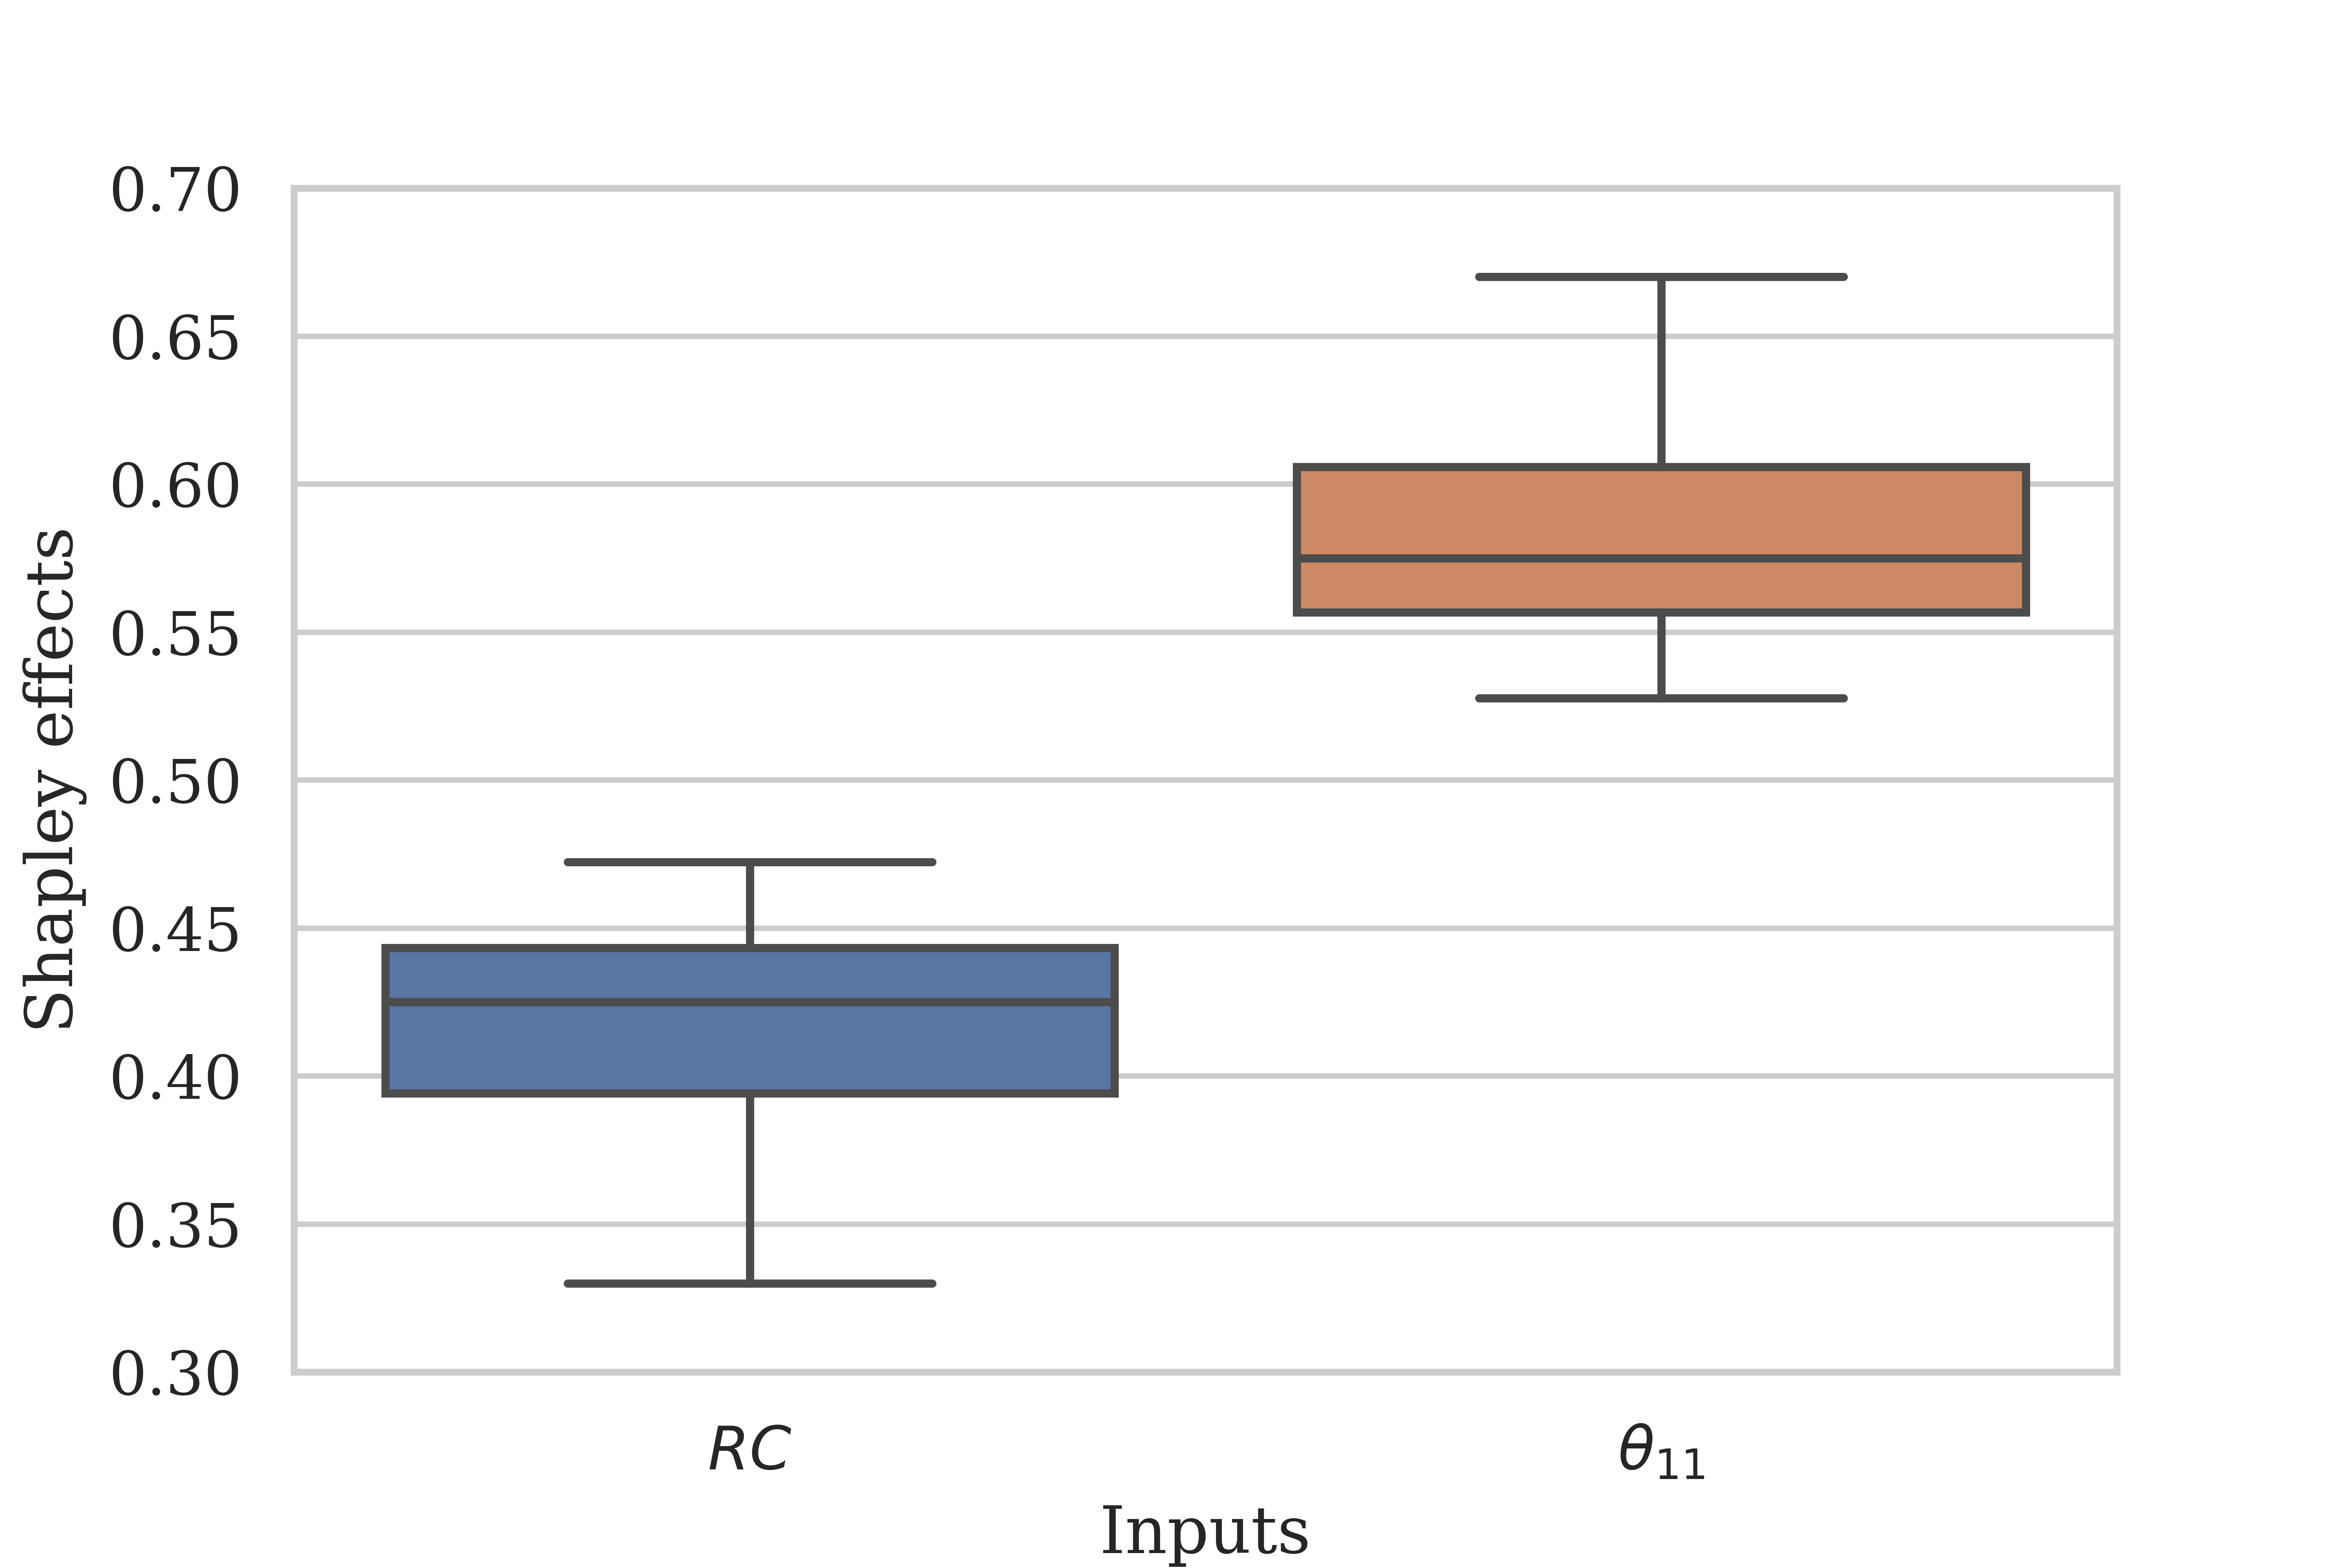
\includegraphics[scale=0.9]{../figures/boxplot_shapley_effects_100.png}

	\end{centering}
	\end{centering}

	\small
	\textit{Notes:} Boxplots for 100 estimated Shapley effects for the inputs $RC$ and $\theta_{11}$ using the same number of Monte Carlo samples: $N_V=100$, $N_O=10$, and $N_I=3$.
\end{figure}

The algorithm for the computation of Shapley effects needs to allow for conditional sampling of dependent inputs. Otherwise, some of the advantages of Shapley effects cannot be exploited. I use algorithm 1 from \citet{SNS16}.\footnote{An alternative algorithm has been recently proposed by \citet{PRB20} which uses mathematically more advanced concepts.}

Shapley effects consider all input subsets. To iterate over all subsets, \citet{SNS16} restate the equation for Shapley effects to iterate over all permutations of model inputs. For instance, let $k=5$. Then, $K=\{1,\ 2,\ 3,\ 4,\ 5\}$. There exist $5!$ permutations, where one example is $\pi'=(2,\ 4,\ 3,\ 5,\ 1)$. Let the set of all permutations of $K$ be denoted by $\Pi(K)$. Further, let $P_i(\pi)$ denote all inputs in permutation $\pi$, that come before input $i$. In the above example, if $i=3$, then $P_3(\pi')=\{2,\ 4\}$. Using the permutation representation, \citet{SNS16} state the marginal contribution due to input $i$ as $val(P_i(\pi) \cup\{i\}) - val(P_i(\pi))$. By considering all permutations of $K$, we can restate the equation for the Shapley effects for input $i$ as
\begin{equation*}
\phi_i=\sum_{\pi \in \Pi(K)} (k!)^{-1} (val(P_i(\pi) \cup\{i\}) - val(P_i(\pi))).
\end{equation*}

The algorithm of \citet{SNS16} exploits the fact that their permutation-based algorithm evades redundant model evaluations by going through the permutations beginning with the smallest subset. The contribution of the preceding subset is subtracted from the contribution of the current subset. The marginal contribution is then computed by writing
\begin{equation*}
val(P_{\pi(j)}(\pi) \cup \{\pi(j)\}) - val(P_{\pi(j)}(\pi)),
\end{equation*}

\begin{table}[t]
	\centering
	\caption{Descriptive Statistics Shapley Effects - $100$ Replicates}
	\label{shapley_descriptives}
	\begin{threeparttable}
	\centering
	\begin{tabular}{lrrrr}
\toprule
{} &    Mean &  Std. errors &  CI lower bound &  CI upper bound \\
Shapley Effect &         &              &                 &                 \\
\midrule
$RC$           &  0.4163 &       0.0043 &          0.4078 &          0.4247 \\
$\theta_{11}$  &  0.5837 &       0.0043 &          0.5753 &          0.5922 \\
\bottomrule
\end{tabular}

	\begin{tablenotes}
	\small
	\item \textit{Notes:} Descriptive statistics for $100$ replicates of the Shapley effects. 95-percent confidence intervals are reported.
	\end{tablenotes}
	\end{threeparttable}
\end{table}

\noindent where $\pi(j)$ denotes the input at position $j$ in permutation $\pi$. In the above permutation $\pi'$, at position 2 we have input 4, i.e. $\pi'(2)=4$.

To see for which subsets the algorithm performs evaluations of $val$, consider the below example. For instance, following \citet{SNS16}, if $k=3$ and $\pi=(1, 3, 2)$, the algorithm computes
\begin{align*}
\Delta_1 &=val(\{1\})-val(\emptyset),\ set\ prevC=0, \\
\Delta_2 &=val(\{1,\ 3\})-prevC,\ set\ prevC=val(\{1,\ 3\}), \\
\Delta_3 &=val(\{1,\ 3,\ 2\})-prevC,\ set\ prevC=val(\{1,\ 3,\ 2\}).
\end{align*}

The algorithm implements three Monte Carlo simulations. There are $N_V$ Monte Carlo samples of model inputs which are evaluated to get an estimate of $V[Y]$. Since the algorithm needs to handle dependent inputs, \citet{SNS16} implement dependent sampling by an inner and an outer Monte Carlo simulation. To see why both Monte Carlo simulations are needed, fix a permutation $\pi$. Then, sample $N_O$ outer samples, that are unconditionally drawn. Given this set of unconditionally drawn outer samples, draw $N_I$ inner samples conditionally on the outer samples. That is, for each outer sample, we has $N_I$ inner samples. Thus, the computational cost in terms of number of model evaluations is given by $N_V+m \cdot N_I \cdot N_O \cdot (k-1)$, where $m$ is the number of permutations considered. In the exact setting of algorithm 1, $m=\vert \Pi(K) \vert=k!$. If only a random subset of permutations should be considered, we set $m<k!$, which can be useful to reduce the computational burden if the number of inputs is large.

\subsection{Shapley Effects for the Rust Model} \label{shapley_rust_model}

I apply three different computational setups. I do so to firstly, evaluate the performance of Shapley effects and, secondly, get the correct input ranking according to the sensitivity for the Rust model. When working with the algorithm presented by \citet{SNS16} in practice, it can be challenging to specify the sample sizes $N_O$ and $N_V$, since no guidance on how to allocate the computational budget to $N_V$ and $N_O$ is given.

The general computational setup applies to all three simulation studies. \citet{SNS16} recommend setting $m=\vert \Pi(K) \vert$, if computationally feasible. In order to reduce variance of the estimates of Shapley effects, they further recommend choosing $N_I=3$, while setting $N_O$ as large as possible, given the constraints on the computational budget. Since the Rust model has two inputs only, the number of permutations to be considered is two and thus very small. Hence, I set $m=2!=2$ and $N_I=3$. I run the estimation by using the implementation of the algorithm by the package \textit{econsa}, a Python package for sensitivity analysis \citep{OSE21}.

% Shapley replicates.

\begin{figure}[t]
	\caption{Convergence of Shapley Effects for the Rust Model}
    \label{shapley_convergence}
	\begin{centering}
	\vspace*{-4mm}
	\begin{centering}
	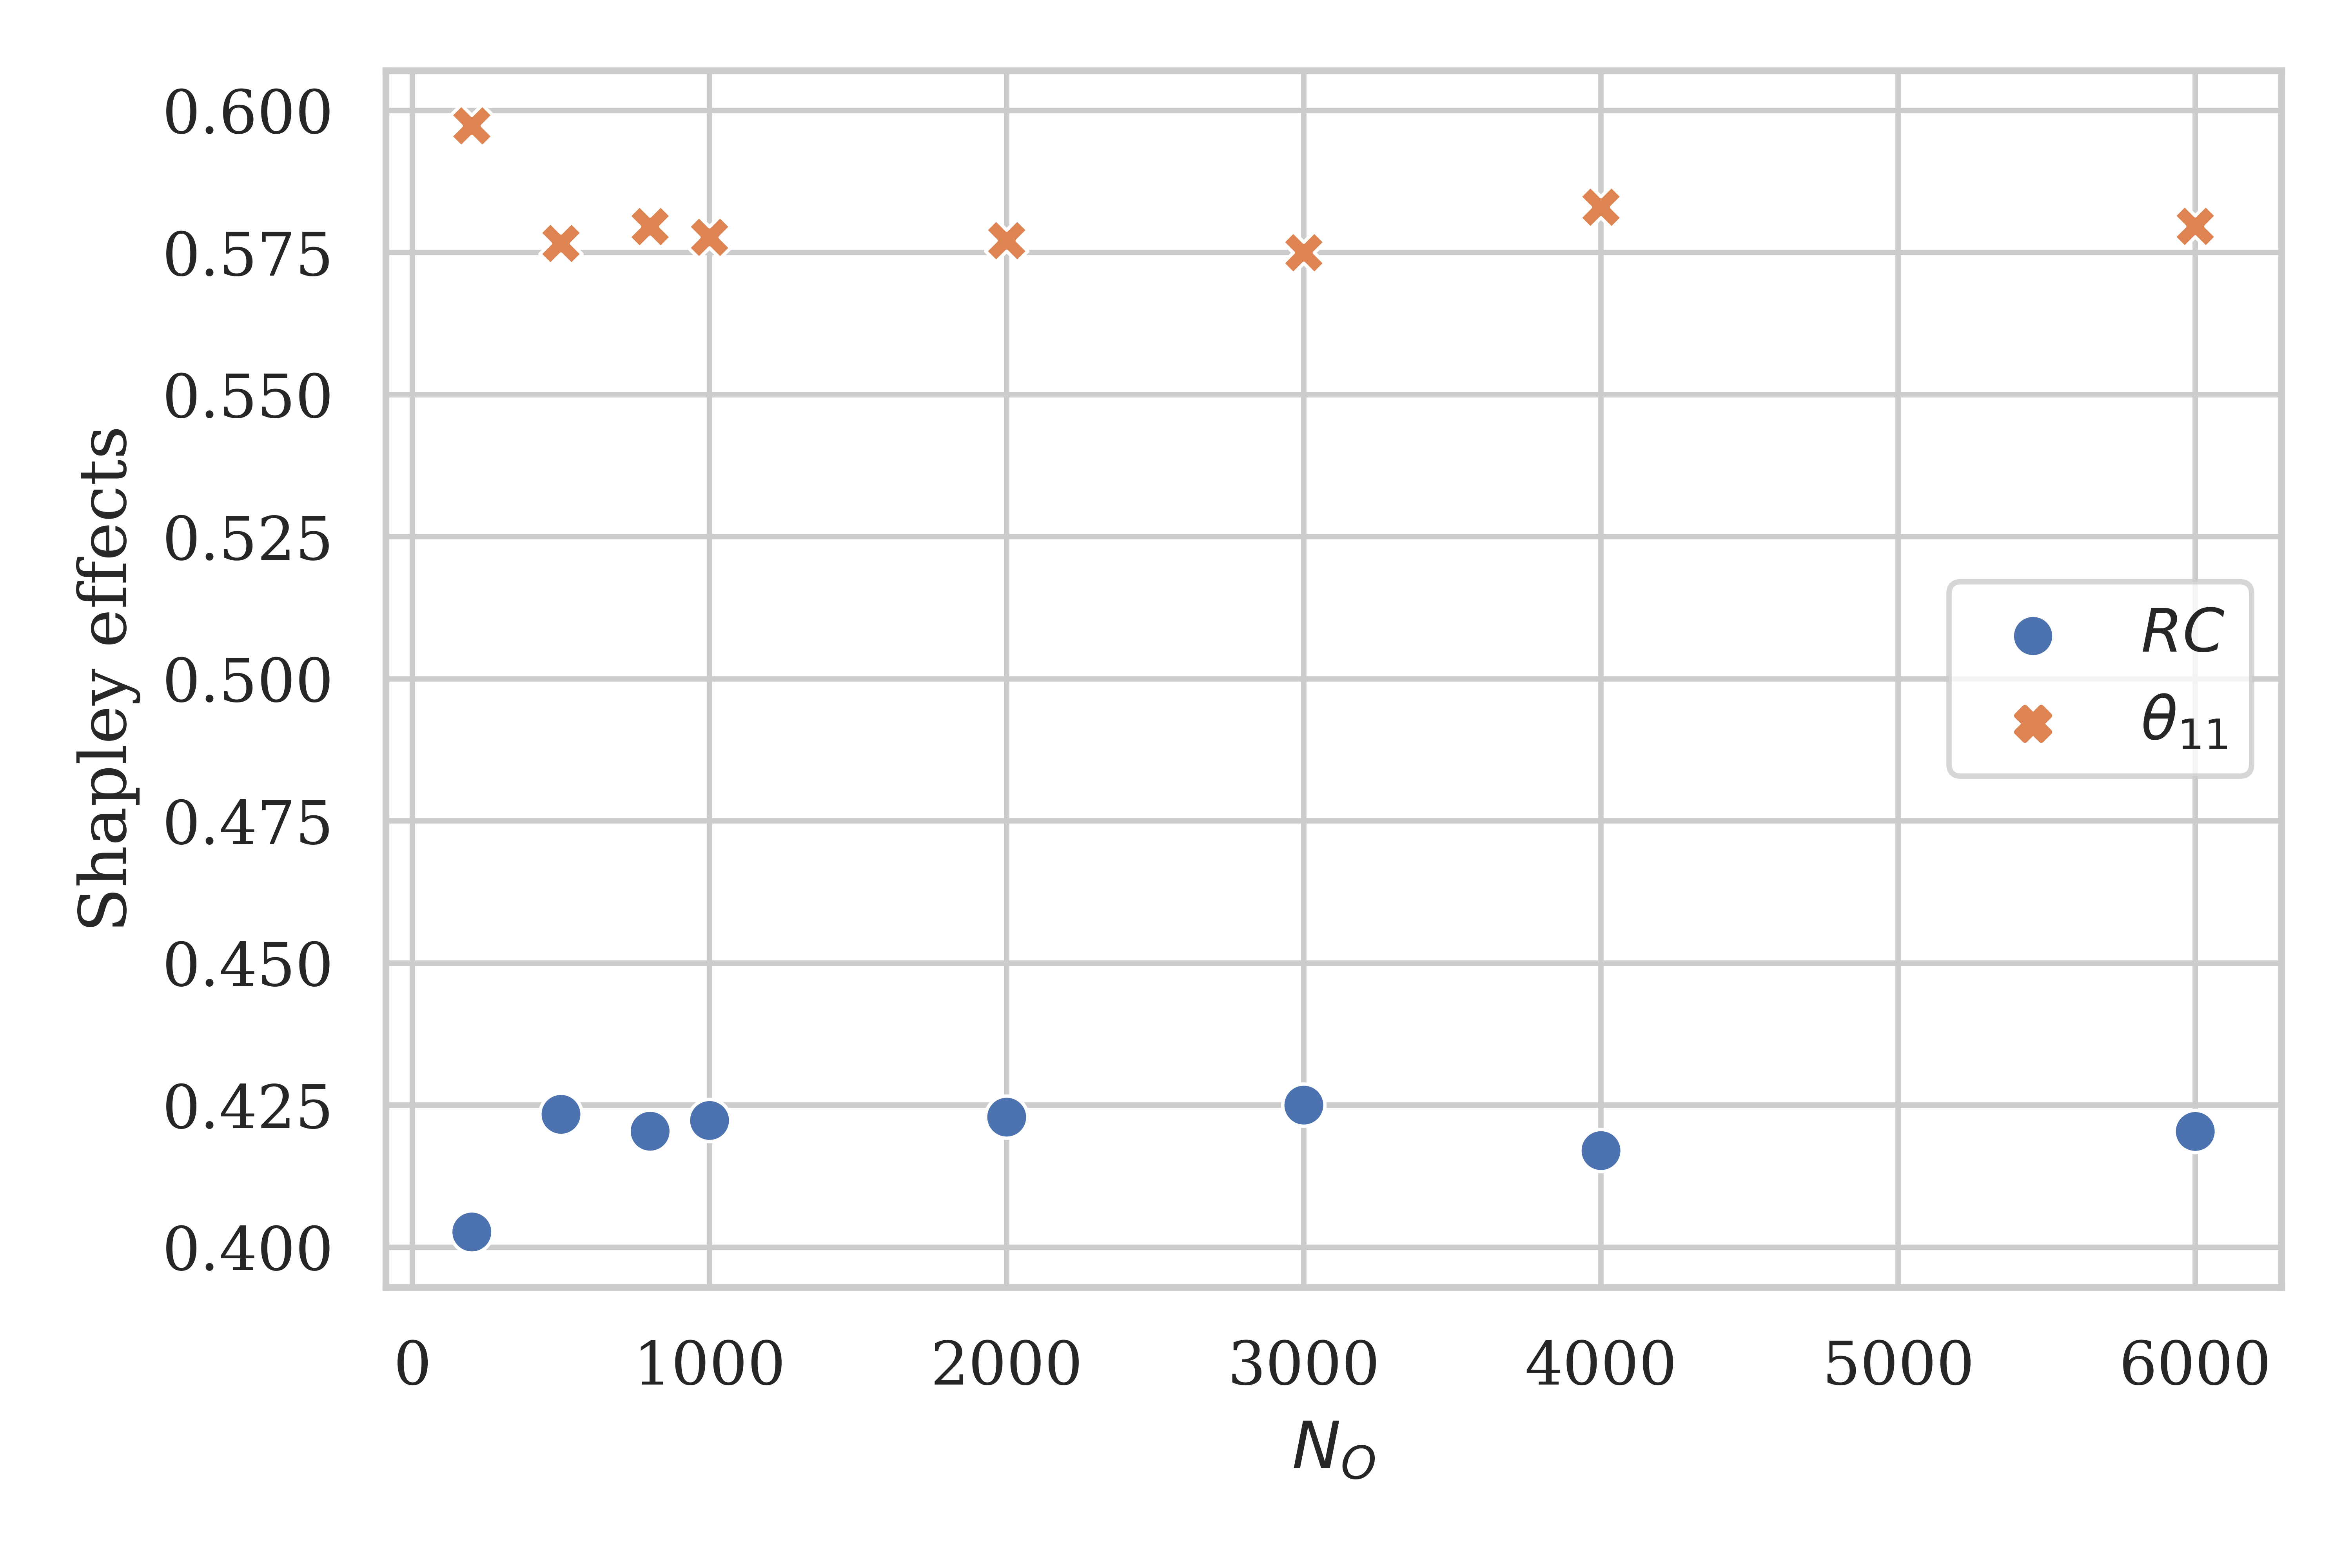
\includegraphics[scale=0.9]{../figures/convergence_shapley_effects_8.png}
	\end{centering}
	\end{centering}

	\small
	\textit{Notes:} Shapley effects estimated for different values of $N_O$, while setting $N_V=10\,000$ and $N_I=3$.
\end{figure}

Firstly, I estimate 100 Shapley effects for the inputs of the Rust model, $RC$ and $\theta_{11}$ using the same general setup as described in the preceding paragraph. I further set $N_V=100$ and $N_O=10$. Thus, the computational cost of my choice of Monte Carlo runs imply that 160 model evaluations are needed to estimate the Shapley effects. On my machine (Windows 10, i5 processor), one estimation run takes approximately 40 seconds.

The distribution of the 100 replicates is visualised by the boxplots in \cref{boxplot_shapley}. For further details on the estimated replicates, see \cref{shapley_descriptives}. The mean of $\phi_{RC}$ is $0.4163$ and for $\phi_{\theta_{11}}$ the mean value is $0.5837$. Shapley effects are estimated with a standard error of 0.0043.
Both, the boxplots, and the mean values show that $\theta_{11}$ is the more important input in terms of contributions to output variance. The confidence intervals at the 95-percent level, are quite large, but they do not overlap, indicating that the implied input importance ranking is robust. The lower value of $\phi_{RC}$ shows that $RC$ has less an impact on the output variance than $\theta_{11}$.

% True Shapley

Secondly, I estimate one set of Shapley effects for a large sample size. I chose to consider $N_V=100\,000$ and $N_O=10\,000$, which amount to a computational cost of $160\,000$ model evaluations. The resulting sensitivity measures are $\phi_{RC} = 0.4176$ and $\phi_{\theta_{11}} = 0.5823$. I refer to this set of sensitivity measures as the \textit{true} Shapley effects.

% Shapley Convergence

Thirdly, I estimate eight Shapley effects for different sample sizes to illustrate their behaviour as $N_O$ increases. For all the estimations I fix $N_V$ at $12\,500$, varying $N_O$ only. I consider $N_O \in \{200,\ 500,\ 800,\ 1\,000,\ 2\,000,\ 3\,000,\ 4\,000,\ 6\,000 \}$. The total computational cost for one estimation is thus given by $10\,000 + 6 \cdot N_O$, e.g. for $N_O=200$, the total computational cost amounts to $11\,200$ and for $N_O=6\,000$, the total computational cost amounts to $46\,000$ model evaluations. Results are visualised in \cref{shapley_convergence}. For each chosen value of $N_O$ there is a clear input ranking, indicating that $\theta_{11}$ is the more important input. Shapley effects are still relatively volatile, even for larger sample sizes. Details on the relative difference between estimates are shown in \cref{rel_diff_shapley}. \Cref{rel_diff_shapley} shows the percentage change in estimates given by $\frac{\phi_i^{n_o-1} - \phi_i^{n_o}}{\phi_i^{n_o}}$, for $i \in \{RC,\ \theta_{11}\}$ and $n_o$ denoting the different values of $N_O$ considered. % Relative differences do not steadily decline.

% Interpretation

To sum up, the input rankings are always the same: $\theta_{11}$ is the more important input for the Rust model. This holds true for all the estimations of Shapley effects presented above. Since both $\phi_i$ are far from zero, it is not recommended to fix any one of them, since both influence the output variance significantly. Otherwise we would assume an input to be deterministic which is subject to large uncertainty and has simultaneously a large influence on the model output.

\begin{table}[t]
	\centering
	\caption{Relative Difference Shapley Effects}
	\label{rel_diff_shapley}
	\begin{threeparttable}
	\centering
	% \hline
	\begin{tabular}{lrrrrrrr}
\toprule
{} &  500  &  800  &  1000 &  2000 &  3000 &  4000 &  6000 \\
Inputs        &       &       &       &       &       &       &       \\
\midrule
$RC$          &  5.14 & -0.70 &  0.45 &  0.14 &  0.50 & -1.88 &  0.81 \\
$\theta_{11}$ & -3.47 &  0.52 & -0.33 & -0.10 & -0.37 &  1.39 & -0.58 \\
\bottomrule
\end{tabular}

	\begin{tablenotes}
	\small
	\item \textit{Notes:} The percentage difference between Shapley effects for different values of $N_O$ while keeping $N_V$ fixed at $12\,500$ and $N_I$ at $3$. Percentage changes are calculated by $\frac{\phi_i^{n_o-1} - \phi_i^{n_o}}{\phi_i^{n_o}}$, for $i \in \{RC,\ \theta_{11}\}$ and $n_o$ denoting the different values of $N_O$.
	\end{tablenotes}
	\end{threeparttable}
\end{table}